\chapter{人工智能核心技术（易炜涵）}
% 一个启下

在第三章中，将深入探索支撑人工智能的核心技术，这些技术是将“人工智能”这一概念从理论推向实际应用的关键。人工智能可以被视为一台强大的机器，而这些核心技术则像是机器的引擎，使其能够在实际环境中运行并完成各种任务。

首先，重点关注“计算机视觉”这一技术，它使机器能够“看懂”世界。计算机视觉是一种通过模拟人类视觉系统的方式，使机器能够从图像和视频中提取信息、识别物体并做出智能决策的技术。在图像识别领域，计算机视觉已取得显著成果，深度学习的应用使机器能够通过分析数百万张图像，自动识别物体、场景和面孔。随着技术进步，计算机视觉广泛应用于医疗影像分析、自动驾驶、视频监控等领域。例如，在医疗领域，计算机视觉通过对医学影像的自动分析，辅助医生进行精准诊断；在自动驾驶领域，计算机视觉通过实时识别道路上的障碍物和交通标志，保障无人驾驶的安全。

接下来，将探讨“语言识别”技术，这项技术使机器能够理解、处理和生成自然语言。语言识别是人工智能技术中最具挑战性的领域之一，涉及到语音识别、自然语言处理（NLP）等多个子技术。自然语言处理技术使计算机能够分析并理解人类语言中的句子结构、语义和情感。例如，智能语音助手和聊天机器人都依赖语言识别技术，通过理解用户的语言输入来做出相应的回答或操作。通过深度学习，语言识别技术已经在语音转文本、机器翻译、情感分析等领域取得显著进展，并在实际应用中展现出巨大的潜力。

最后，关注“生成式人工智能”技术，它赋予机器创造和生成内容的能力。生成式人工智能包括生成对抗网络（GANs）和变分自编码器（VAEs）等模型，使机器能够生成真实感极强的图像、音频、文本等内容。一个典型的应用是生成式AI在艺术创作中的应用，AI可以通过学习已有的艺术作品风格，创作出新的图像、音乐或文本，甚至模仿某些艺术家的创作风格。生成式人工智能还在深度伪造（Deepfake）、虚拟人物和游戏设计等领域中展现出独特潜力。

通过深入了解这些核心技术，可以看出，人工智能并不仅仅是一个抽象的概念，而是由多个技术组成的复杂系统。每一项技术的进步都推动人工智能在现实世界中发挥着越来越重要的作用。从智能医疗到自动驾驶，从智慧城市到个性化推荐，人工智能的核心技术不仅正在改变着生活方式，也在不断提升处理复杂问题的能力。

本章将对这些技术进行详细分析，揭示它们如何实现基本任务，并展示它们在各行各业中的实际应用。通过对核心技术的了解，将更加深入地认识人工智能如何从基础任务走向应用，从理论走向现实，并在未来发挥越来越大的作用。

\section{计算机视觉：让机器看懂世界}

想象你走进一个陌生的房间，四周的物品看起来新奇且陌生。你首先看到桌上的计算机、热咖啡和几本书。这些物品你能迅速识别并理解它们的用途：计算机用来工作，咖啡用来提神，书本提示这里可能是一个学习或工作的地方。接着，你的目光移向墙上的一幅画，色彩鲜艳，细节生动，增添了艺术气息；窗外透进阳光，照在地面上，带来温暖而宁静的感觉。

这一切你都能迅速理解，这得益于你大脑和眼睛的强大视觉处理能力。你不仅能分辨物体的形状、颜色和大小，还能推测它们的用途和相互关系。你“看见”了物体，并理解它们的功能和它们之间的关系。

但如果是计算机来观察这个房间，它能像你一样理解这些物品和场景吗？这就是\textbf{计算机视觉（Computer Vision}）要解决的核心问题。计算机视觉是让计算机能够从图像或视频中获取信息并进行理解的技术。它的目标不仅仅是识别图像中的物体，还要让计算机能够理解这些物体的功能、它们之间的空间关系以及它们所处的语境。

具体来说，计算机视觉就是通过计算机技术，让计算机模仿人类的视觉感知，识别图像中的物体、场景以及它们之间的关系，并做出智能决策。你在房间中看到的“计算机”、“咖啡”和“书本”不仅仅是物体，它们代表了特定的功能和作用——计算机是用来工作的，咖啡帮助提神，书本则暗示这里是一个学习空间。计算机视觉的任务就是让计算机不仅识别出这些物体，还能理解它们的功能，以及它们在整个环境中的作用。

为了实现这一目标，计算机需要不仅识别物体的颜色、形状和纹理，还要能够理解更高层次的含义。例如，计算机需要知道“计算机”通常和“书本”一起出现在学习或工作环境中，而“咖啡”则作为辅助工具，帮助保持清醒。计算机不仅要推测物体之间的关系，还要理解它们在空间中的布局，以及它们如何共同作用，影响整个房间的氛围。

与传统的图像处理方法不同，计算机视觉的任务远不止是“看见”物体，它还要求计算机理解物体的意义，以及它们如何互相关联。比方说，计算机需要识别“桌子”和“椅子”之间的空间关系，推测它们是用来工作还是休息的。这种理解需要计算机具备强大的感知和推理能力。

为了让计算机具备这种理解能力，通常使用深度学习和神经网络等技术。这些技术通过大量的数据训练，使计算机逐步学会识别物体的特征，理解它们之间的复杂关系，从而实现更高层次的图像理解。

计算机视觉的应用已经遍布各个领域。从自动驾驶汽车的路标识别，到智能手机的面部识别，再到医学影像分析，计算机视觉的技术正深刻地影响着我们的生活。随着技术的不断发展，未来计算机将能够更精准地理解世界，帮助我们做出更智能的决策。让我们从计算机视觉的诞生讲起。

\subsection{计算机视觉的奠基者}

在1960年代的一个寒冷冬夜，伦敦的一个实验室里，一位年轻的科学家正对着桌上的计算机显示屏凝视。他的眼前没有闪烁的星光，也没有丰富的自然景象，只有一个充满公式和数据的屏幕。大脑依旧是他的探索目标，但他并不满足于仅仅依赖观察来获取知识，他渴望通过数学的力量揭示视觉如何在大脑中运作。

此时他心中疑问着：“我们是如何看见这个世界的？大脑如何从一片光线与阴影中提取出有意义的物体、场景和深度？”他反复思考这个问题，试图从自然界的神经科学研究中找到启示。那时，神经科学家如David Hubel\footnote{David Hubel（1926--2013）是加拿大出生的美国神经生物学家，因其在视觉神经科学方面的开创性研究获得诺贝尔生理学或医学奖。他与Torsten Wiesel共同研究了视觉皮层的功能，并提出了关于视觉信息处理的分层理论。}和Torsten Wiesel\footnote{Torsten Wiesel（1924--）是瑞典神经生物学家，因其与David Hubel合作研究大脑视觉皮层的功能，揭示了神经元如何处理视觉刺激而获诺贝尔奖。他们的研究为理解大脑如何处理视觉信息提供了重要线索。}正在研究大脑如何处理视觉信息。他们发现，大脑中的视觉皮层在处理视觉刺激时，特定的神经元负责不同的任务——例如，一些神经元专门识别边缘，有的则专注于深度感知，而其他神经元则负责颜色和运动的处理。这一发现向科学界展示了视觉信息处理的层次性：视觉并非由单一部分进行，而是由多个阶段、不同的区域和不同类型的神经元协同工作。

这一研究启发了年轻科学家的思考：“如果大脑是通过这种分层的方式来处理视觉信息，那么计算机能否也模仿这种结构？”他想，如果计算机能够分阶段、逐步地理解图像，可能就能像人类一样“看见”世界。

于是，他开始构思如何设计一个分层的计算机视觉系统。对于他来说，这不仅是一个科学问题，也是一个哲学性的问题：计算机是否也能像人类一样理解视觉信息？如果可以，它又如何分层理解这些信息？

这位科学家在构建他的视觉系统时，借鉴了当时神经科学和认知科学的最新成果。他逐渐形成了三层次的计算机视觉模型，并将其视为理解“计算机视觉”这一复杂问题的关键：

\begin{itemize}
    \item \textbf{计算理论层次}：首先，他定义了计算机视觉的目标。它不仅仅是简单地捕捉图像，更重要的是理解图像中传递的信息，如物体、深度、形状等。他认为，计算机视觉的真正挑战在于如何让计算机理解视觉信息，而不仅仅是处理图像。
    
    \item \textbf{表示与算法层次}：在这个层次，他开始思考如何在计算机内部有效地表示这些视觉信息，并设计合适的算法来处理这些信息。每个物体、每个边缘，每一条线条，都需要一种恰当的数学表示。而计算机则需要具备识别这些复杂信息结构的能力。通过这一层次的思考，计算机才能逐步理解和“看到”图像的结构。
    
    \item \textbf{硬件实现层次}：最后，考虑到计算机仅仅通过“算法”是不够的，他还必须思考这些算法如何在实际的计算机硬件上实现。这意味着要设计合适的传感器和硬件来采集和处理视觉信息，让计算机具备“看见”的能力。他提出，计算机视觉不仅仅是关于算法的事，还涉及到感知系统的构建，包括图像输入设备和图像处理的硬件。
\end{itemize}

在这个过程中，他不仅受到了神经科学的启发，还受到一些计算机科学领域大牛的影响。例如，他深入研究了Alan Turing的计算理论\footnote{Alan Turing（1912--1954）是英国数学家、逻辑学家、密码学家，被誉为计算机科学之父。他提出的“图灵机”模型奠定了计算理论的基础，并为破解第二次世界大战中的德国密码提供了关键帮助。}和John McCarthy的人工智能理论\footnote{John McCarthy（1927--2011）是美国计算机科学家，人工智能领域的奠基人之一。他提出了“人工智能”这一术语，并创造了LISP编程语言。McCarthy的研究影响深远，特别是在智能系统和机器学习方面。}，这些理论为他提供了关于如何构建智能系统的深刻启示。他不仅从生物学中借鉴了神经元的分层组织，还借用了计算机科学中的分层思想来构建自己的视觉处理模型。通过结合生物学与计算机科学的知识，他创造了一个全新的计算机视觉框架。

他将这些思考汇总成了自己的著作《视觉》（Vision: A Computational Investigation into the Human Representation and Processing of Visual Information），在书中，他详细阐述了这一层次化的视觉处理框架，并提出了计算机视觉不应仅仅被看作是一个单一的图像处理问题，而是应该通过多层次的系统逐步解决。从图像的低级特征提取，到更高层次的形状识别、立体视觉，再到最后的对象识别和场景理解，计算机视觉的处理过程应该是逐步复杂化的。
\begin{figure}[htb]
	\centering
	
\includegraphics[width=0.5\linewidth]{image/3/vision.jpg}
\end{figure}


这些想法不仅改变了计算机视觉的研究方向，也为未来的人工智能研究和视觉识别技术的发展提供了新的视角。许多科学家和工程师受到了他的启发，推动了机器视觉、人工智能和计算机视觉技术的发展。通过这些理论，计算机能够更准确地理解视觉信息，推动了自动驾驶、面部识别、图像分类等领域的进步。

尽管他在1980年因病早逝，但他对计算机视觉领域的贡献却永远铭刻在历史中。年轻的科学家通过把数学、神经科学和计算机科学融合起来，揭示了计算机如何“看见”世界的秘密。这位年轻科学家，正是 David Marr，他的三层次视觉模型成为了计算机视觉的基石，影响了无数后来者。



\begin{figure}[htb]
	\centering
	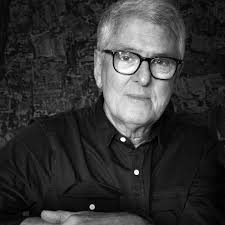
\includegraphics[width=0.75\linewidth]{image/3/David Marr.jpg}
	\caption{David Marr}
\end{figure}

随着计算机技术的不断发展，\textbf{计算机图形学}作为人工智能（AI）的一部分，逐渐成为一个独立且不断演进的研究领域。最初，计算机视觉主要集中在简单的图像处理任务上，但随着技术的进步，它已经发展成一个涵盖多个方面的复杂领域。如今的计算机视觉不仅仅局限于图像分析，还涉及到让机器“理解”图像和视频内容，并广泛应用于各个实际场景。

在计算机视觉的发展过程中，研究者们提出了多种分类方式，以帮助更好地理解这个庞大的领域。以下是一些常见的分类维度\footnote{本节中提出的计算机视觉分类维度参考自 ACM Computing Classification System，该系统为计算机科学各领域提供了一种标准化的分类方式，帮助研究者和学者更好地理解和讨论不同技术和方法的关系。}：

\begin{enumerate}
    \item \textbf{计算机视觉任务}（Computer Vision Tasks） \\
    计算机视觉任务是指如何让计算机在实际环境中“看见”并理解图像或视频内容。任务更关注“做什么”，即具体应用或功能的目标。任务本身通常是用户或应用系统所需的高层目标。例如，\textbf{物体检测}（找出图像中的物体）、\textbf{图像分类}（把图像归类到不同类别）、\textbf{场景理解}（理解图像中不同元素的关系）等任务，都是通过计算机视觉技术解决的实际问题。而为了完成这些任务，通常需要解决多个相关的技术问题，例如图像分割、目标识别等。这些技术问题构成了完成任务的基础。

    \item \textbf{计算机视觉问题}（Computer Vision Problems） \\
    计算机视觉问题更关注“如何做”，即实现任务时需要解决的具体技术或算法难题。例如，\textbf{图像分割}（将图像分成多个有意义的部分）、\textbf{目标识别}（识别图像中的特定对象）、\textbf{跟踪}（追踪移动物体）等问题，都是计算机视觉领域中的关键难题。问题是任务的组成部分，任务本身可以是较高层次的目标，而问题则是实现该目标所需解决的低层次技术难题，仍然是当前研究的重点。
    
     \item \textbf{计算机视觉表示}（Computer Vision Representations） \\
    这部分关注如何表示图像中的结构和特征。例如，计算机如何通过\textbf{特征点}、\textbf{边缘}、\textbf{纹理}等信息来表达图像中的内容，使得计算机能够有效地理解这些图像。这样的表示方式为计算机分析图像提供了重要的线索。

    \item \textbf{图像与视频采集}（Image and Video Acquisition） \\
    这部分关注如何从物理世界中采集图像和视频数据。它不仅涉及到\textbf{摄像头}、\textbf{传感器}等硬件设备的设计与优化，还包括如何通过这些设备有效捕捉世界中的动态和静态信息。这是计算机视觉能够“看到”世界的基础。为了实现这些目标，通常需要解决相关的技术问题，如如何提高图像质量、如何减少采集误差等，这些问题与任务密切相关，构成了该子领域的研究内容。
\end{enumerate}


随着这些不同维度的发展，计算机视觉在学术界取得了显著进展，并逐渐渗透到各个行业的应用中。例如，\textbf{自动驾驶}（让汽车自主感知周围环境）、\textbf{医疗影像分析}（帮助医生通过图像诊断病变）、\textbf{智能监控}（实时分析监控视频中的活动）等领域，都依赖计算机视觉技术来提供支持。

本节将在后续小节中，通过一些经典的计算机视觉案例，深入讲解这些任务、表示、问题和技术背后的基本原理和实际应用，帮助读者更好地理解计算机视觉的最新进展与挑战。


\subsection{计算机视觉任务与问题的典例}

想象一下，你走进一个繁忙的机场，四周是匆匆忙忙的旅客，巨大的电子屏幕不断闪烁着航班信息。你走到安检处，工作人员挥手示意你走向一台自助人脸识别系统。你站在那里，短短几秒钟，系统便确认了你的身份，自动打开了安检门。无需排长队、无需检查身份证，只要你站在那里，它就能识别你是谁。

这个看似简单的过程，背后却隐藏了一个复杂的技术任务——人脸识别。要完成这一任务，计算机需要解决一系列问题。首先，它需要从一张复杂的图像中识别出人脸。这就像是在人群中快速找到一个特定的人一样，而计算机则需要从五光十色的背景中准确捕捉到每一张人脸。

接下来，计算机还要确认这个人脸属于谁。这不仅仅是对比照片那么简单，因为人脸在不同的光照、角度或表情下会有不同的表现。因此，计算机需要提取出人脸的“特征”，这些特征能够在不同环境下帮助识别出同一个人。就像是iPhone上的Face ID，设备通过扫描用户的脸部特征来解锁手机，背后采用的技术便是深度学习和计算机视觉中的特征提取和人脸比对技术\footnote{Face ID技术：iPhone上的Face ID系统通过深度学习和计算机视觉技术，利用红外线扫描、三维面部扫描以及深度学习算法，提取用户面部特征并进行比对，从而实现手机的安全解锁。这种技术的应用不仅限于手机，还在支付和身份验证等多个领域发挥作用。}。

尽管现在的人脸识别技术已经非常成熟，但在一些特殊情况下，比如低光环境或者某些人的面部特征模糊，系统依然会遇到困难。这就像iPhone在你戴着口罩时无法识别你的脸，或者机场的人脸识别系统无法在昏暗的灯光下准确辨识。这些技术挑战让人脸识别的应用场景更具复杂性，因此在人脸识别背后，我们看到的不仅仅是一个图像识别的问题，还是对光照、角度、细节等多方面挑战的攻克。

接着，从人脸识别到自动驾驶，计算机视觉的任务范围和技术难度不断拓展。在自动驾驶场景中，计算机视觉的要求变得更加复杂。想象一下，你坐在一辆无人驾驶的汽车里。车子没有司机，只有你和车载的显示屏。车子启动后，它开始自动行驶，沿着路面行进，不时进行加速、减速或转弯。这辆车不仅仅是按预设的路线行驶，它还会不断地“看”周围的环境，避免与其他物体发生碰撞。

这一切，正是计算机视觉在自动驾驶中的应用。自动驾驶汽车要完成的任务是：让汽车安全、智能地行驶。为了做到这一点，车子需要理解它周围的环境。比如，它需要能够检测到前方的行人、路边的障碍物，甚至其他驶过的车辆。这就是计算机视觉中的物体检测与障碍物识别的关键应用。

特斯拉的自动驾驶系统便是这样一个例子。特斯拉通过配备摄像头、雷达和激光传感器来感知周围环境。这些传感器不断扫描周围的物体，并将信息传输给车载计算机。然后，计算机利用图像识别技术分析这些传感器数据，判断前方是否有行人、车辆或障碍物，并做出相应的反应\footnote{特斯拉的多传感器系统：特斯拉的自动驾驶系统通过融合来自摄像头、雷达、激光雷达（LiDAR）等多个传感器的数据，形成一个完整的环境感知图像。这些传感器能够实时监测道路上的物体和障碍，提升车辆的安全性。}。

例如，特斯拉的系统需要能够实时识别出行人并计算他们与车辆的相对位置。如果前方有人走到车道中，系统会迅速计算出该行人是否可能与车辆发生碰撞，从而触发紧急制动。而这一过程依赖的正是计算机视觉中的实时物体跟踪与预测技术。

然而，自动驾驶所面临的挑战并不仅限于白天的清晰天气。在晚上或雾霾天气中，汽车的摄像头和传感器可能会受到影响，视线变得模糊。就像你在雾天开车时，肉眼无法清晰看到远方的物体，自动驾驶系统也会面临类似的困境。因此，如何让汽车在复杂的天气条件下依然能够准确识别路况，成为了一个技术难题。

为了应对这些问题，特斯拉不仅仅依赖摄像头，它还结合了多个传感器，如雷达和超声波传感器，这就像是你在遇到视线受限时，不仅依赖眼睛，还可以用耳朵和触觉来感知周围环境。这种多传感器融合的方式，能够在不同条件下提高对环境的感知能力。汽车通过将来自不同传感器的信息整合，增强了系统的准确性，使它能够更精确地识别并做出判断。

随着技术的发展，计算机视觉不仅仅停留在“识别”层面，它已经在不断渗透到我们生活中的方方面面。从人脸识别到自动驾驶，技术不断进步，让我们感受到计算机能够“看”得更清楚，也能够做出更聪明的决策。无论是iPhone的Face ID，还是特斯拉的自动驾驶，每一项技术的背后，都离不开复杂的计算机视觉处理，它们的成功展现了如何从图像中提取信息、分析环境，并在多变的现实世界中做出智能的决策。
\subsection{计算机视觉的其他内容}

在上一节，我们探索了计算机如何通过计算机视觉“看懂”世界。但是，想要让计算机理解它看到的东西，其实是个非常复杂的过程。如果我们把计算机视觉比作是给计算机装上一双眼睛，那么这个过程就像是让它不只是“看见”世界，还要学会“理解”世界中的每一个细节。那么，假设一下，如果计算机突然拥有了无数双眼睛，它能如何快速理解和应对周围的环境呢？

\begin{itemize}
    \item \textbf{假设情境一：如果计算机能像我们一样快速理解图像，它会如何识别世界？}  

    想象一下，计算机突然获得了像人类一样的视觉能力，不仅能看见物体，还能立刻知道那是什么东西——苹果、杯子，还是你刚刚放在桌上的饼干。我们看到一张图片时，瞬间就能判断其中的物体。可是对计算机来说，图像其实只是由无数个像素点组成的数字矩阵。要理解这些图像，它得先把这些数字“翻译”成对我们有意义的东西。

    这个翻译过程就像你读书时，快速理解书中的内容一样——首先得识别字母，接着理解单词，再到句子，最后明白整篇文章的意思。计算机通过特征提取，找出图像中的边缘、颜色、纹理等信息，就像我们看书时识别封面和排版来判断书的主题一样。经过深度学习的训练，计算机最终能识别出图像中的物体，判断它们是苹果还是杯子，甚至是那只你不小心丢在桌上的橙子。

    \item \textbf{假设情境二：如果摄像头变得不完美，计算机又该如何适应？}  

    再假设一下，如果摄像头突然变得不再完美，光线太强或者环境过于复杂，计算机又该怎么办？比如，在夜晚或恶劣天气条件下，图像变得模糊不清，计算机就像眼睛模糊的我们一样，根本无法清晰地识别物体。我们如何应对呢？我们依赖增强光线、放大视野，或者依赖我们的大脑进行猜测和推理。

    同样，计算机在图像采集过程中也会遇到类似的挑战。它们通过光学传感器将光线转化为电子信号生成图像，但是如果图像信息不清晰，计算机就可能无法作出准确判断。在这种情况下，计算机必须通过深度学习技术，像我们一样进行反复“训练”，从而变得更加适应不同的环境。

    \item \textbf{假设情境三：如果计算机能像人类一样做决策，它会如何处理复杂的场景？}  

    再想象一下，如果计算机不仅能识别图像，还能像我们一样，基于所看到的做出决策。在自动驾驶场景中，计算机需要“看”到路标、行人、车辆，并且决定是该加速、减速还是转弯。如果突然遇到一个障碍物或者其他不可预见的情况，计算机如何快速分析并作出反应？如果它判断错误，是不是会撞到路上的“路障”——比如你正在路边走的猫？

    计算机做决策的过程其实和我们判断交通情况是类似的。我们通过视觉、听觉和直觉判断交通状况，然后做出加速或刹车的决定。计算机通过图像识别技术，先识别出图像中的物体，然后根据这些信息判断当前的行车环境。在自动驾驶中，计算机通过从大量的训练数据中学习，逐渐建立起一个“交通规则库”，从而能够在复杂的交通环境中做出迅速的反应。
\end{itemize}

通过这些假设情境，我们可以看到计算机视觉技术背后的复杂性。计算机通过“眼睛”——也就是图像采集设备，获得信息，然后通过一系列的算法和模型，将这些原始数据转化为能够理解和决策的有用信息。虽然这一过程涉及复杂的数学和技术，但计算机视觉正在改变我们的生活，从智能手机到自动驾驶，再到医疗影像分析，计算机视觉的应用正悄悄地进入我们的每一个角落。未来，随着技术的不断进步，我们可以期待计算机在更多场景中展现它的智慧与能力。

在这方面，像华为这样的技术公司也在不断推进计算机视觉的实际应用，尤其是在自动驾驶和智能监控等领域。华为通过深度学习等先进技术，提升了视觉系统在复杂环境下的识别能力，使其能够在光线不足或视觉信息模糊的情况下，依然保持高效的性能。这种技术的发展，使得计算机不仅能“看”得更清楚，还能在动态环境中做出快速反应，为许多行业带来了革命性的改变。

\subsection{总结}

在第3.1节中，我们深入探讨了计算机视觉技术的基本原理及其广泛的应用。从让机器“看懂”世界的挑战，到如何通过深度学习和神经网络使计算机理解图像中的物体、场景及其关系，我们揭示了计算机视觉的核心任务和实现路径。计算机视觉不仅仅是图像处理，它要求机器能够理解图像背后的深层含义，进而做出智能决策。通过不断的技术进步，计算机视觉已经在自动驾驶、医疗影像分析、视频监控等领域取得了显著成果，正在深刻改变着我们的生活方式。

通过对计算机视觉的讨论，我们可以看到，人工智能的发展离不开各项核心技术的相互支持和推动。计算机视觉技术的进步为其他人工智能领域提供了强有力的支持，也为我们理解世界、提升生产力和创造力提供了更多的可能性。在下一节中，我们将继续探讨另一项至关重要的人工智能技术——语言识别，进一步揭示人工智能在理解和生成自然语言方面的潜力与挑战。


\section{语音识别}


你有没有过这样的体验？想让你的语音助手播放一首你喜欢的歌，结果它为你选了一首让你想当场拔掉电源的曲子？你心情愉快地说“调高温度”，它不仅没有加热，反而把空调给关掉了，简直让你怀疑自己是不是生活在一个冰天雪地的家里。更糟糕的是，当你尝试用浓重的口音或者在吵闹的环境中与语音助手互动时，你会发现自己所有的努力都付之东流——它完全听不懂你在说什么。你清楚地讲出“打开音乐”，但它竟然播放了一个令人崩溃的广告。有没有想过，为什么这些看似简单、直白的命令，总是被机器听得“云里雾里”？你是否曾幻想过科幻电影中的语音助手，那种能像人类一样理解复杂命令、灵活应对的助手，然而现实却给了你一个“硬邦邦”的回应：系统无法识别你的命令。嗯，看来，听懂人类的语言，计算机仍然有一段很长的路要走。那么，问题到底出在哪里呢？为什么这样一个看似简单的“语言”任务，对于计算机来说，竟然如此复杂？

\subsection{如何听到？}

为了破解这个谜团，我们需要先从语言的复杂性谈起。语言，乍一看，似乎是一种非常自然、容易理解的东西，但实际上它比我们想象的要复杂得多。语言不仅仅由一个个字词组成，它背后隐藏着无数的语音信号，而这些信号又受到诸多因素的影响。举个例子，假设你说“你好”，不同地区的人会用不同的口音和音调发音。北京人说的“你好”和上海人说的“你好”，就像两个完全不同的音符——即使这两个词完全一样，也因为发音的细微差别，使得它们的声音听起来就像两首不和谐的钢琴曲。而且，除非你真的有一种超能力，否则你是无法理解别人方言中的“你好”的。再比如，假如你在安静的房间里说话，语音助手能轻松地听清你的指令；但在嘈杂的街道上，哪怕你大声疾呼，它也可能连你的嘴巴在动都听不见。这就是为什么，尽管语言是我们每天都使用的工具，计算机却总是面临着“听错”的困扰。每一次语言交流都充满了不确定性和变数——你甚至可以说，语言就像一场极具挑战性的智力游戏，充满了陷阱和难题。

\subsubsection{语音识别的基础}

那么，语音识别系统是如何处理这些复杂的信号的呢？它的第一步就是将“语言”从声音信号中提取出来，换句话说，就是“把声音变成数字”。听起来是不是很魔幻？但实际上，计算机并不直接听你说话，它把声音转换成了一系列的数字，接着通过这些数字来理解你的意图。这个过程通常被称为“声音的数字表达”，包括两个关键步骤：采样和量化。采样是把连续的声音信号切成一个个小片段，然后将每个片段转化为数字；量化则是对声音的振幅进行精确的测量，使得计算机能从无数的波动中“听”出规律。

\subsubsection{采样：声音的“切片”}

想象一下，你正在和朋友一起去吃披萨。你们正在聊着天，突然，服务员走过来说：“你们要不要试试我们的新口味披萨？”你急忙抬头，用眼睛扫视四周——你注意到那个披萨是由很薄的饼皮和一层层的配料组成的。你有点饿，于是决定就试试这道“神秘披萨”。

接下来，你看到了一块正好能塞进你嘴巴的小披萨片。你决定拿下这一片，感受它的美味。你不需要吃整块披萨，吃上一小片就能大概判断它的味道。实际上，你拿到的只是披萨的一个切片。

好啦，现在我们把这个比喻转换一下，想象声音就是“披萨”。声音波形是一个连续的信号，但我们不需要每一秒钟都去“吃”整个信号的“披萨”。于是，计算机用采样的方式，把声音的波形“切”成一个个小片段，每个片段叫做一个采样点。通过这些切片，计算机可以根据不同的“口感”来判断出整体声音的特征。

这个切片的大小，就是“采样率”。如果你用一个较大的切片，那么你吃到的披萨味道会很“粗糙”，可能很难分辨出细节；但如果你每次都切得很细，你的判断就会更加准确，能更好地“捕捉”到每一片披萨的味道。

例如，如果你想要每秒采样1000次，那么采样率就是1000 Hz。如果你想要更高的精度，你可以选择更高的采样率，就像你希望每次切下一片更小的披萨一样。但是，采样率太高也不是好事，因为计算机要处理更多的数据，可能就会慢下来，甚至吃不消。因此，如何选择一个合适的采样率，就是每个语音识别系统要面临的“披萨选择题”——太低了会丢失信息，太高了会让系统过载。

了解了采样的基本概念后，我们接下来需要探讨的是量化过程，它同样在声音数字化中扮演着至关重要的角色。

\subsubsection{量化：音量的“测量”仪}

现在，想象你手中拿着一个量杯，准备给你的朋友倒饮料。你倒了几次，但每次倒的量都不一样——一次倒满、一次倒半满、一次倒得很少。你突然意识到，这样倒饮料根本没办法让每个人都喝到一致的量！于是你决定，采用一个标准化的量杯，每次倒酒的时候，都严格按照标准来倒。

量化的过程，其实就是这样的一个“标准化”过程。当计算机通过采样将声音切成了一个个片段后，它需要测量每个片段的“音量”。但是，声音的波动是连续的，就像你倒饮料时可以随意倒出任何量的酒。但是，计算机的“量杯”必须是有限的——它只能选择一定的数值范围。例如，它只能分成 8 个等级（8-bit量化），或者 16 个等级（16-bit量化）。这些数值范围就像“量杯”一样，把声音的音量按照不同的标准进行“量化”。

量化的目标是将声音的连续信号转变成数字信号，并且要尽量保留原始声音的特征。就像量杯在倒酒时要尽量保持倒的量一致一样，量化要尽量准确地表示每个声音片段的强度。如果量化精度低，可能会导致信号失真，像倒酒时你没有按标准量杯倒酒一样，味道就会变得不准确。

例如，8-bit的量化会把音量分成 256 个等级，16-bit 的量化则能提供 65536 个等级。如果你用16-bit量化，系统就能更精确地表达声音的波动，就像你用更精确的量杯来倒饮料时，朋友们就能喝到差不多相同的量。不过，像每秒采样1000次，每次量化16bit的量杯，这样的操作会使得计算机的工作量增大——换句话说，它需要处理更多的数字信息。

\subsubsection{采样与量化的博弈：选择正确的量杯与切片}

在语音识别中，采样与量化是两个至关重要的过程，它们如同层层叠加的选择题，直接影响着最终的识别效果。采样是将声音信号在时间上离散化，而量化则是将这些离散的信号在幅度上离散化，转化为计算机可以处理的数字信号。

选择过低的采样率或量化的精度不足，会导致声音信号的失真，就像通过模糊的画面判断披萨的味道，无法还原真实的声音。反之，选择过高的采样率和量化精度，虽然能提供更准确的声音细节，却会带来计算资源的浪费和效率低下，如同将披萨切得过于细碎。

因此，采样和量化之间需要找到一个平衡点，既能高效地捕捉声音的关键信息，又不会让系统不堪重负。这种平衡是在速度与准确性之间的完美妥协，是一个持久的研究话题。

在采样方面，低比特率语音编码技术如MELP和EVS，通过降低传输带宽需求，保证了语音质量，成为语音识别的重要研究方向。例如，Alan McCree开发的MELP编码器被广泛应用于低比特率语音通信，并成为北约标准。

在量化方面，Geoffrey Hinton和邓力将深度神经网络引入语音识别，显著提升了量化的精度和系统性能。尽管这些技术取得了突破性进展，但仍面临语言多样性和复杂环境的挑战，如口音和噪声问题。当前研究正探索基于神经网络的语音增强技术，以提高系统的鲁棒性。

而这一切的突破，离不开深度神经网络在语音识别中的引入。 深度神经网络不仅改变了量化的方式，还彻底革新了语音识别的整体框架，使其从传统的基于规则的方法转向了数据驱动的智能化模式。接下来，我们将重点讲述深度神经网络是如何改变语音识别这一领域的。


\subsection{如何听清？}

在原有的语音识别技术中，传统方法面临的挑战主要在于对不同口音、方言以及复杂噪音环境的适应能力。例如，经典的语音识别系统大多基于隐马尔可夫模型（HMM）和高斯混合模型（GMM），这些方法通过预设的规则与词库进行语音匹配。这种方式的局限性在于，它无法灵活地应对口音变化、背景噪音、语速加快等变化，识别准确度受到许多因素的影响。

深度神经网络（DNN）在语音识别中的应用彻底改变了传统的技术框架，特别是在处理复杂语言特征和噪声问题上的表现。传统的语音识别系统依赖于预先设定的规则和词库，这些系统将音频信号转化为数字特征，并与词库中的发音模板进行比对。然而，这种方法面临许多挑战，尤其是对不同口音、语速变化和背景噪音的处理。

不同地方的发音差异使得传统系统难以适应。例如，北京口音和上海口音的“吃饭”在发音和韵律上有所不同，传统系统很难准确识别。此外，嘈杂的环境（如街头或多人交谈的房间）常常干扰信号的清晰度，导致识别错误。同样，语速较快或变化较大的讲话也会使得传统系统处理起来困难重重。

深度神经网络（DNN）通过大规模数据训练自动识别语音信号中的复杂模式，提供了解决这些问题的革命性方法。与传统方法不同，DNN并不依赖于人工设计的规则，而是通过模拟人类大脑的神经网络结构，逐层提取音频信号中的特征，从而逐步建立对语言的理解。

DNN的多层结构使其能够逐层提取音频信号的特征。最初的层关注低级音频特征，如音调、频率和音高，类似于人耳最初感知到的声音特征。接下来的层关注音节、语音单元（如元音和辅音的结合）等较为抽象的特征，而更高层次则关注语句的结构和语境信息。例如，在识别“吃饭”时，网络会理解这是指吃东西，而不是去餐馆吃饭。

DNN能够自动适应不同的口音和语速，因为它通过大量的语音数据进行训练。系统并不需要人为编写规则来处理不同的发音，而是通过学习多种发音方式的共性来识别不同口音的词汇。无论是普通话、粤语还是带有地方特色的方言，DNN都能根据训练数据调整识别策略，从而提高识别的准确性。例如，当一个上海人用带有上海话口音的英语发音“hello”时，DNN能够识别出这个词，而不会误认为其他词汇。

对于嘈杂的环境，DNN通过特征学习提高了噪声鲁棒性。通过训练含有噪声的语音数据，DNN能够忽略背景噪音，专注于提取有效的语音信息。例如，在一个嘈杂的街头环境中，DNN能够从人群和车流的声音中识别出“我要买票”这一语音信号，而不会被背景噪音所干扰。相比之下，传统语音识别系统往往会因噪音而识别错误。

除了声音特征外，DNN还能够通过上下文信息提升识别精度。这种上下文感知能力帮助系统理解同音词和相似发音的区别。例如，在“我去买菜”这句话中，DNN不仅能识别单词，还能通过上下文推断每个词的意义，以确保准确的语句理解。

深度神经网络的引入，使得语音识别从传统的基于规则的匹配方法转变为基于数据学习的识别方法。通过多层次的特征提取，DNN能够自动适应不同的口音和语速，并在噪声环境中保持较高的鲁棒性。这种能力使得DNN在语音识别领域具有显著的优势，能够处理更为复杂和多样的语言特征。

尽管DNN在语音识别领域表现出了强大的潜力，但依然面临挑战，特别是在极端噪声环境和复杂语言情境下。随着更多创新技术的引入，语音识别技术将变得越来越智能，能够应对更多复杂的语言识别任务。

如果你希望进一步了解深度学习的原理和在语音识别中的应用，推荐阅读以下资料：
\begin{itemize}
    \item \textit{《深度学习》}（Ian Goodfellow, Yoshua Bengio, Aaron Courville） — 深度学习的权威教材，涵盖了神经网络的基础和应用。
    \item \textit{《语音与语言处理》}（Daniel Jurafsky \& James H. Martin） — 一本全面讲解语音识别与自然语言处理的书籍，非常适合对语音识别原理有深入兴趣的读者。
\end{itemize}



\subsection{如何听懂？}

随着技术的不断发展，卷积神经网络（CNN）和循环神经网络（RNN）陆续加入了语音识别领域。这些神经网络模拟了人类大脑的神经元工作原理，通过不同的方式更好地捕捉语音的时序性和上下文信息。具体来说，卷积神经网络能够有效地识别音频中的局部特征，比如音节或发音的模式，而循环神经网络则擅长捕捉语音中的时间序列信息，理解语言背后的上下文关系。

这些技术的加入，极大地增强了语音识别的准确性和鲁棒性。比如，Google DeepMind推出的WaveNet模型，通过模拟人类发音的方式，不仅提高了语音识别的自然度，还能够捕捉语音中的情感、语气等信息。例如，当你紧张地说出“开空调”，WaveNet能够“理解”你背后的情绪，快速做出响应，而不仅仅是机械地执行命令。WaveNet甚至可以根据你的情绪变化，调节语音助手的回应语气，让语音助手变得更加“贴心”，不再是一个冷冰冰的执行工具。

进入到“大模型时代”，语音识别技术迎来了更加深刻的变革。在这一时代，像ChatGPT-4这样的大规模语言模型不仅在文本生成方面展现了超凡的能力，也为语音识别技术提供了新的动力。ChatGPT-4等大模型的成功，得益于其庞大的参数量和对上下文的深刻理解，这使得它能够在更复杂的语言任务中提供极为精准的预测和回应\footnote{ChatGPT-4等大模型的成功，得益于其庞大的参数量和对上下文的深刻理解，使得它们能够提供精准的预测和回应。}。

随着深度学习技术的发展，尤其是Transformer模型的出现，语音识别系统的架构发生了根本性变化。在大模型时代，语音识别不再是单纯地将语音转换为文字，而是进入了一个更加深度的“理解”阶段。像ChatGPT-4这样的模型具备了强大的上下文推理和长文本理解能力，能够在处理语音时，不仅识别出说话的内容，还能根据语境进行合理的推断。

例如，在传统的语音识别中，机器可能会对多义词或含糊的语句做出错误的理解，产生不准确的转录结果。而大模型能够通过对上下文的理解，消除这些歧义。例如，当你说出“我想吃苹果”，而系统正好处于关于健康饮食的对话中，大模型能够正确理解你是在谈论水果，而不是公司名称“苹果”。这种上下文理解能力，极大提升了语音识别的精准性和灵活性。

不仅如此，大模型还具备了多模态学习的能力。通过结合图像、音频、视频等多种信息来源，它能够更好地理解和解析语音背后的多维信息。在语音识别中，这意味着不仅仅依赖纯粹的声音特征，系统还能够借助视觉信息（例如面部表情）或情境信息（例如语音背景）来增强对语音内容的理解。如此一来，语音识别不仅限于语言文字的转换，而是扩展到了更广泛的语境分析和情感推断。

在语音助手和智能客服领域，大模型的加入使得机器能够理解情感、语气和潜在意图，从而实现更加个性化的语音交互。比如，虚拟助手不仅能够识别你说的话，还能够理解你说话时的语气和情绪状态。当用户愤怒地说出“为什么这么慢？”时，大模型能够理解用户的不满情绪，并作出相应的安抚回应，而不仅仅是机械地告诉用户“系统正在处理”。

大模型不仅提升了语音识别的准确性，还推动了语音识别的质量提升。在传统的语音识别中，系统往往对复杂的发音、口音或背景噪音敏感，导致识别错误频发。而现在，得益于大规模模型的训练，语音识别系统能够适应更多的方言、音调变化以及复杂的语音环境。即便是在嘈杂的街道或车内，系统也能保持较高的识别精度。

此外，随着大模型的不断迭代，语音识别系统的响应速度和实时性也得到了提升。过去，语音识别需要耗费大量计算资源，导致延迟较高，而如今，大模型的高效推理能力使得系统在提供高精度识别的同时，依旧保持了良好的实时性。

这种技术的突破，使得语音识别不仅仅停留在“理解”层面，它已经进入了“理解并回应”阶段。今天的语音识别技术不仅能够识别指令，还能理解意图、推断情绪、并做出人性化的回应。随着大模型和深度学习技术的不断发展，语音识别已经不再局限于简单的命令控制，它扩展到了自动语音翻译、语音客服等多个领域。这使得我们的生活变得更加智能和便捷。

而最重要的是，在这一技术的推动下，我们已经不再需要面对那些“死板”的机器回应，今天的语音助手能够通过理解我们的情绪，作出更加自然、流畅和人性化的互动，仿佛它已经学会了“聆听”并“回应”我们真实的需求。随着大模型的广泛应用，语音识别将会成为我们日常生活中不可或缺的一部分，成为智能时代的一项标志性技术。

\subsection{总结}
通过这个引人入胜的故事，我们见证了语音识别技术从“听到”到“听清”，再到“能够理解”的伟大转变。这个过程的背后，是无数工程师和科学家的不懈努力，他们不断突破技术瓶颈，将一个个看似不可能的任务变成了现实。技术的进步使语音识别不再仅仅停留在“听到”声音的阶段，而是逐渐走向了“能够理解、反馈、甚至与人产生情感共鸣”的全新境界。

也许，下次你再与语音助手互动时，它不仅能准确理解你的需求，甚至能够察觉你语气中的微妙情绪变化，并给予你更加贴心的回应。这一切，正是深度学习和神经网络技术带来的奇迹。



%\subsection{离线与实时语音识别}

%语音识别可分为离线识别和实时识别两种模式。离线识别通常在本地设备上完成，具有快速响应和隐私保护的优势，而实时识别则依赖网络资源，通过云端服务器进行高精度计算，且能够持续更新数据，但对网络环境有较高的要求。
%\begin{itemize}
   % \item \textbf{离线识别}：适用于没有网络连接或隐私要求较高的场景。
  %  \item \textbf{实时识别}：依赖云端计算资源，适用于需要高准确度和不断优化的应用场景。
%\end{itemize}

\section{生成式人工智能}

本节，我们将介绍生成式人工智能技术。最好的方式，就是通过一段段我与 AI 的对话，让大家亲身体验这一技术的魅力！通过这次互动，我们不仅能感受到生成式人工智能的独特之处，还能深入了解其背后的原理和应用。目的是帮助大家更好地理解这一颠覆性技术，并探索它如何改变我们的世界。

\begin{quote}
我说：\\
我是一名作者，正在写一本关于人工智能的科普书，想要在书中介绍生成式人工智能。你能帮我简单概括一下这个技术吗？

ChatGPT 说：\\
生成式人工智能（Generative AI）是一种利用机器学习技术，特别是深度学习模型，生成新的、符合一定规律的数据内容的技术。这些内容可以是文本、图像、音频、视频等。生成式模型的核心是通过大量的训练数据，学习到数据中的结构和规律，从而能够根据输入的条件生成新的、看似原创的内容。

常见的生成式AI技术包括：

\begin{itemize}
  \item \textbf{生成对抗网络（GANs）}：由两个神经网络（生成器和判别器）相互对抗，生成器尝试生成尽可能真实的内容，而判别器则评估这些内容的真实性，最终生成器能够生成非常逼真的图像或其他类型的内容。
  \item \textbf{变分自编码器（VAEs）}：通过编码器将数据压缩成潜在空间，再通过解码器生成新的样本，常用于图像生成。
  \item \textbf{自回归模型（如GPT、BERT等）}：这些模型在处理文本时，能根据输入的部分内容生成剩余部分，广泛应用于自然语言生成、翻译、摘要等任务。
\end{itemize}

生成式AI的应用领域非常广泛，除了创作艺术作品、自动写作，还能用于虚拟角色创建、数据增强、模拟数据生成等多个行业。
\end{quote}


这段对话\footnote{所有对话内容是通过与 ChatGPT 模型的互动生成的，模型为通用版本，没有进行任何特殊的定制或调整。生成的内容基于预先训练的大规模数据集，并通过自然语言处理技术提供回答。 }展示了生成式人工智能技术的基本概念和一部分关键词。接下来，我们将进一步探讨其历史背景和发展历程。



\subsection{发展简史}

生成式人工智能（Generative AI）在过去几十年中经历了多个技术突破和里程碑事件，这些突破推动了其从基础的概率模型到如今复杂的多模态生成技术的演变。以下是生成式人工智能技术的关键发展节点：

\begin{quote}
我说：那生成式人工智能的发展史是如何的呢？经历了哪些大事件？

ChatGPT 说：\\
生成式人工智能（Generative AI）的发展历史可以追溯到几个重要的技术突破和里程碑事件。以下是一些关键发展节点：

\begin{enumerate}
  \item \textbf{早期的概率模型（20世纪50-70年代）}：
  概率模型与贝叶斯推断：早期的生成式模型基于概率论，尤其是贝叶斯网络和马尔可夫过程。此时期的重点是如何生成数据分布并通过统计方法模拟真实世界数据。
  
  \item \textbf{神经网络的初步探索（1980-1990年代）}：
  神经网络的崛起：神经网络在80年代得到了初步应用，尤其是多层感知器（MLP）和反向传播算法的提出，为后来的深度学习和生成式模型的发展奠定了基础。
  限制玻尔兹曼机（RBM）：一种概率生成模型，能够在无监督学习中从数据中抽取特征，尤其在图像生成任务中有较早的应用。

  \item \textbf{生成对抗网络（GANs）的提出（2014年）}：
  Ian Goodfellow提出GANs：2014年，Ian Goodfellow等人在《生成对抗网络》论文中提出了生成对抗网络（GANs），这标志着生成式AI的一个重大突破。GANs通过两个神经网络——生成器和判别器——进行对抗训练，从而生成具有极高质量和真实感的图像和其他数据。这一突破让生成式AI在计算机视觉、艺术创作等领域得到了迅猛发展。

  \item \textbf{变分自编码器（VAE）和深度生成模型（2014年）}：
  VAE的提出：与GANs同步，变分自编码器（VAE）也在2014年由Kingma和Welling提出。VAE是另一种深度生成模型，通过优化变分下界来学习潜在空间，从而生成数据。VAE与GANs的主要区别在于其生成方式是通过编码-解码架构，而不是对抗训练。

  \item \textbf{自回归模型和大型预训练语言模型（2018年起）}：
  GPT系列（2018年起）：OpenAI推出的GPT（Generative Pretrained Transformer）系列模型，特别是GPT-2和GPT-3，基于Transformer架构，能够生成高质量的文本。GPT系列标志着生成式AI在自然语言处理（NLP）领域的突破，使得文本生成和语言理解达到了新的高度。  
  BERT与T5模型：Google提出了BERT（Bidirectional Encoder Representations from Transformers）和T5（Text-to-Text Transfer Transformer），虽然这两者是主要用于理解任务，但它们也在生成任务中取得了显著进展。

  \item \textbf{跨领域生成式AI应用（2020年代）}：
  图像生成：随着GANs、VAE、以及Diffusion Models（扩散模型）等技术的发展，生成式AI开始能生成非常真实的图像。比如，DeepMind推出的BigGAN，OpenAI的DALL·E等，都能根据自然语言描述生成图像。
  DALL·E和CLIP（2021年）：OpenAI发布了DALL·E，它能够根据用户输入的文本描述生成图像，而CLIP则将图像和文本结合起来，为生成式AI带来了跨模态（文本-图像）的潜力。

  \item \textbf{深度学习大规模应用和商用化（2020年代初至今）}：
  生成式AI的普及应用：随着计算力的提升，生成式AI逐渐进入主流应用。GPT-3及其商业化应用（如聊天机器人、内容生成等）推动了生成式AI在各行各业的广泛应用。特别是通过OpenAI、Google、Meta等公司的努力，生成式AI技术已经在多个领域取得突破性进展，包括艺术创作、广告、游戏开发、甚至科学发现等。
  扩散模型（Diffusion Models）：近年来，扩散模型成为生成式AI的新宠。像Stable Diffusion和MidJourney等工具，利用扩散模型生成高质量的图像，这些工具逐渐成为艺术家和创作者的必备工具。

  \item \textbf{多模态生成式AI（2023年起）}：
  多模态生成模型的融合：当前，生成式AI不仅仅局限于单一模态（如文本或图像），而是迈向多模态模型的整合。例如，OpenAI的GPT-4已经能够同时处理文本、图像、音频等多种输入，并生成相应的输出。这使得生成式AI可以应用于更加广泛和复杂的任务中，比如视频生成、虚拟角色创建等。
  
\end{enumerate}

\textbf{发展趋势与挑战：}

\begin{itemize}
  \item 合成内容的伦理问题：随着生成式AI的进步，深伪技术（deepfake）、版权和隐私问题成为重要的社会议题。
  \item 解释性和透明性：尽管生成式AI的结果非常强大，但其“黑箱”性质依然令人担忧，如何使其决策过程更加透明和可解释是当前的研究热点。
  \item 高质量、个性化生成：未来的生成式AI可能会进一步优化个性化创作，能够根据用户需求创造出定制化的内容。
\end{itemize}

总之，生成式人工智能从早期的统计模型到深度学习时代的多样化应用，经历了显著的技术突破，并迅速推动了多个领域的创新与发展。
\end{quote}

在人工智能的各类技术中，生成式人工智能无疑是近年来最引人注目的领域之一。虽然我们可以从AI的回答中提炼出许多关键信息，这些信息无疑是准确且有价值的，但我仍然希望从个人的视角进一步阐述一些问题，并探讨这些技术如何对现实世界产生深远影响。

进入21世纪20年代，生成式人工智能不再仅仅是一个学术研究的边缘话题，它已经开始渗透到我们生活的方方面面。这一切的背后，离不开扩散模型和多模态模型的迅速崛起，它们无疑标志着这一领域的一次质变。

以Stable Diffusion和DALL·E 2为代表的扩散模型，在图像生成技术上打开了一扇新的大门。通过在数据中引入噪声并在反向过程中去除噪声，这些模型实现了高质量图像的生成。相比生成对抗网络（GANs）和变分自编码器（VAEs），扩散模型的可控性和稳定性无疑更具优势，提升了生成图像的质量和效率。

随着GPT-4等多模态模型的出现，生成式AI已经突破了单一模态的限制，跨足了更广阔的应用领域。AI不仅可以生成图像，还能通过文字、图像、声音等多种形式进行深度交互，开辟了虚拟现实、跨媒体创作等前所未有的应用场景。其深刻的影响，不仅限于技术本身，更在于它改变了我们理解和生成信息的方式。

然而，随着技术的不断进步，生成式AI也带来了不少挑战。首先是计算资源的消耗。训练这样庞大的模型需要巨量的算力，这不仅让资源的分配变得更加紧张，还可能加重对环境的负担。其次，AI模型的偏见问题也一直备受关注。即使在技术不断优化的今天，如何确保AI输出的公平性和透明度，依然是一个难以回避的话题，尤其是在涉及敏感问题的领域。

未来，生成式AI可能会在多个领域取得进一步突破，尤其是随着更高效的模型架构的出现，其应用前景不可限量。更重要的是，随着跨学科合作的推进以及伦理和安全问题的逐步解决，AI的社会影响将更为深远。而接下来，我要具体了解生成式人工智能的不同分支的区别。

\subsection{不同的分支}
随着科技的迅猛发展，生成式人工智能已经不仅仅是一个科幻概念，它逐渐渗透到了我们日常生活的各个层面。无论是自动生成的文本、语音合成，还是让机器创作的图像和视频，生成式AI的应用正在从实验室走向实际，影响着许多行业的格局。面对这样一个迅速变化的领域，许多人可能会有这样一个疑问：这些不同形式的生成式AI技术有什么异同？它们各自面临哪些挑战？它们如何通过独特的技术架构，推动着整个领域的革新？为了帮助大家更好地理解这一问题，下面我们将深入探讨文本生成、音频生成、图像生成、视频生成和多模态生成之间的差异及其核心技术。

\begin{quote}
\textbf{我说：} 请你简单描述一下文本生成，音频生成，图片生成，视频生成，多模态生成的区别以及对应的核心技术？

\textbf{ChatGPT说：}  
生成式人工智能在不同领域的应用有着显著的差异，每种生成任务都有其独特的技术要求和核心方法。以下是文本生成、音频生成、图片生成、视频生成和多模态生成的简要描述及其核心技术。

1. \textbf{文本生成}  
核心技术：自回归模型（如GPT系列）、变换器（Transformer）、BERT、T5等。

特点：文本生成的目标是根据给定的输入（如提示词或上下文）生成自然、流畅的语言文本。文本生成模型通常基于大规模语料库进行训练，学习语言的结构和语法规则。  
核心技术：GPT（Generative Pretrained Transformer）、BERT、T5等基于Transformer的架构，能够有效捕捉上下文依赖关系，生成连贯的文本。  
应用场景：自动写作、聊天机器人、机器翻译、摘要生成、问答系统等。

2. \textbf{音频生成}  
核心技术：WaveNet、Tacotron、VAE、GANs。

特点：音频生成主要指通过模型生成自然的语音或音乐。生成的音频内容需要模拟人类发音或乐器声音，要求模型在时间序列上具有高精度。  
核心技术：WaveNet是基于深度神经网络的语音生成模型，能够生成高质量的自然语音。Tacotron等模型则常用于语音合成，通过将文本映射到语音波形来生成音频。VAE和GANs也可以用于音频生成，尤其是在无监督学习场景下。  
应用场景：语音合成（TTS）、音频增强、音乐生成、虚拟助手。

3. \textbf{图片生成}  
核心技术：生成对抗网络（GANs）、变分自编码器（VAE）、扩散模型（Diffusion Models）。

特点：图片生成技术需要模型生成符合自然规律的图像，如人物、风景等。模型不仅要理解图像的结构，还要确保生成的图像具有高度的真实感。  
核心技术：GANs通过生成器和判别器的对抗训练生成图片。VAE在图像生成中通过潜在空间生成图像，扩散模型则通过逐步去噪来生成图像。最近，扩散模型如Stable Diffusion和DALL·E等取得了很大成功。  
应用场景：艺术创作、图像修复、虚拟角色生成、风格迁移等。

4. \textbf{视频生成}  
核心技术：GANs、RNN（递归神经网络）、时序生成模型（如TGAN、MoCoGAN）。

特点：视频生成除了涉及图像生成的挑战外，还需要考虑时序和动态信息。生成的视频需要在时间维度上保持一致性，保证物体运动流畅。  
核心技术：时间生成对抗网络（TGAN）、MoCoGAN等，结合了GAN和RNN或其他时序模型，能够生成动态变化的图像序列。通过学习时序特征，模型可以生成具有连贯性的动作或场景。  
应用场景：虚拟现实、动画制作、深伪视频、影视特效。

5. \textbf{多模态生成}  
核心技术：CLIP、DALL·E、VQ-VAE、跨模态对抗生成模型。

特点：多模态生成是指同时处理和生成多种类型的数据（如图像、文本、音频等）。例如，根据文本描述生成图像，或根据图像生成文本描述。多模态生成涉及到不同模态之间的转换与对齐。  
核心技术：CLIP（Contrastive Language-Image Pre-training）通过对比学习将文本与图像结合。DALL·E结合了GPT和VQ-VAE，能够根据文本生成图像。跨模态生成模型如T5可以处理多种输入和输出模态，生成多种类型的内容。  
应用场景：图文生成（如DALL·E）、视频描述生成、跨模态检索（如图像搜索文本）等。

总结：  
文本生成：主要依赖自回归模型和Transformer架构，任务聚焦在生成连贯的语言。  
音频生成：通常基于WaveNet、Tacotron等模型，侧重于语音和音频的时间序列生成。  
图片生成：利用GANs、VAE、扩散模型等生成高质量的静态图像。  
视频生成：需要处理时序信息，通常结合GANs和时序模型（如RNN）生成动态内容。  
多模态生成：涉及不同类型数据（如文本与图像）的互相转换，核心技术为跨模态对比学习和多模态预训练模型。  
每种生成任务的技术都有独特的挑战，但都基于深度学习的核心原理，尤其是神经网络的训练与优化，推动了生成式人工智能在各个领域的创新和应用。
\end{quote}
在生成式人工智能（AI）中，涉及到许多复杂的技术名词，可能让初学者感到困惑。为了帮助大家更好地理解这些技术，我们将通过通俗易懂的方式，对其中的一些核心概念进行解释。

\subsubsection*{生成对抗网络（GANs）}
生成对抗网络（Generative Adversarial Networks，简称GANs）是一种由两个神经网络组成的模型：一个生成器和一个判别器。生成器的任务是创造“假”图像或音频，而判别器的任务是判断这些图像是否真实。通过这种对抗过程，生成器不断提升自己的能力，直到生成的内容几乎无法被判别器区分出来。GANs通常用于图像、音频和视频的生成，广泛应用于艺术创作、游戏开发和虚拟现实等领域。

\subsubsection*{变分自编码器（VAE）}
变分自编码器（Variational Autoencoders，简称VAE）是一种通过编码器和解码器网络来生成内容的模型。VAE首先将输入数据（比如图像）压缩成一个“潜在空间”表示，然后通过解码器从这个潜在空间重建出图像。与GANs不同，VAE更注重从数据中提取特征，并通过这些特征生成新的数据。VAE常用于图像生成和图像修复等任务。

\subsubsection*{扩散模型（Diffusion Models）}
扩散模型（Diffusion Models）是一类新兴的生成模型，主要通过逐步“去噪”来生成图像或其他数据。简单来说，它首先将真实的图像加上随机噪声，直到完全变成噪声，然后再通过模型一步步去除噪声，逐渐恢复到一个新的、相似的图像。近年来，基于扩散模型的图像生成技术（如Stable Diffusion）取得了显著突破，被广泛应用于艺术创作、广告设计等领域。

\subsubsection*{自回归模型（Auto-Regressive Models）}
自回归模型是一种常见的生成模型，特别是在文本生成中非常重要。它的工作原理是，模型根据前面生成的内容（例如前几个单词）来预测下一个内容。以GPT系列为例，GPT（Generative Pre-trained Transformer）通过大量语料库的训练，学会了如何根据上下文预测下一个单词，从而生成连贯、自然的文本。自回归模型的优点是生成的内容逻辑连贯，但有时可能会在长文本中出现一些语义上的不一致。

\subsubsection*{变换器（Transformer）}
变换器（Transformer）是一种深度学习模型，它特别擅长处理序列数据（如文本、音频或时间序列）。与传统的循环神经网络（RNN）不同，Transformer通过“自注意力”机制，能够在处理输入数据时考虑到所有位置的信息，而不仅仅是前一个位置的信息。这使得Transformer在长文本生成中表现出色。著名的文本生成模型，如GPT系列和BERT，都是基于Transformer架构的。

\subsubsection*{CLIP（Contrastive Language-Image Pretraining）}
CLIP是一种结合了图像和文本的多模态预训练模型。它通过对比学习（Contrastive Learning）让模型理解文本与图像之间的关联。比如，CLIP能够理解“猫”的图像和与之对应的文字描述“a cat”之间的关系，从而实现根据文字生成图像，或者根据图像生成文字描述。CLIP的出现为多模态生成（如图文生成）开辟了新的方向。

\subsubsection*{TTS（Text-to-Speech）}
TTS（Text-to-Speech）是一种文本转语音的技术，旨在将输入的文字信息转换为自然的语音。常见的TTS技术如WaveNet和Tacotron，通过分析文本中的语调、节奏和发音，生成与人类语音极为相似的音频。TTS广泛应用于智能助手、导航系统和盲人辅助工具中。

\subsubsection*{VQ-VAE（Vector Quantized Variational Autoencoder）}
VQ-VAE是一种结合了自编码器和量化的生成模型。它通过将图像或音频数据转换为离散的“码本”来进行生成。与传统的VAE相比，VQ-VAE通过引入向量量化来提高生成内容的质量和多样性，广泛应用于图像生成和音频生成等任务。

\subsubsection*{总结}
通过理解这些关键技术，我们可以看到生成式AI不仅仅是在复制已有的数据，而是通过学习数据中的规律，创造出全新的内容。这些技术的结合和进步，推动了各行各业的创新，也使得我们有了更丰富的创作工具和方式。随着这些技术的不断发展，AI生成内容的质量和多样性将进一步提升，甚至有可能在未来改变我们的创作和工作方式。

在探索生成式AI的过程中，我不禁回想起自己初次接触这些技术时的心情。那时，听到GPT系列能够“写出”几乎与人类无异的文章，我既震惊又兴奋。我清楚地记得，当时我尝试让一个文本生成模型创作关于人工智能的科幻故事，结果生成的内容不仅结构完整，还带有些许出人意料的创意，这让我彻底改变了对AI的认知。随着技术的不断演进，我又开始接触到音频和图像生成的应用，甚至在一些设计项目中，利用Stable Diffusion等图像生成工具，为自己的PPT设计增添了一抹不同的色彩。这一切让我深刻体会到，虽然每种生成任务的核心技术各不相同，但它们共同推动着人工智能从“工具”向“创造者”转变的过程。而随着多模态生成技术的出现，这一转变变得愈加明显。如今，我们看到的不仅是各类单一模态的生成技术，而是跨越多种数据类型的深度融合，它们正以前所未有的速度、深度与复杂度，改写着创意的边界。



\section{总结与习得技能}

通过本章节的学习，我深刻理解了人工智能核心技术在各个领域中的应用和发展趋势。无论是在计算机视觉、语音识别，还是在生成式AI的创作领域，AI技术的不断创新正在改变我们的生活和工作方式。通过对这些技术的深入了解，我能够更好地应用这些技术，进一步提升我的学习与实践能力。

\section*{生成式人工智能 - 练习题}

\subsection*{选择题}

\begin{enumerate}
    \item 生成式人工智能的主要技术包括：
    \begin{enumerate}[A.]
        \item 支持向量机、随机森林、决策树
        \item 生成对抗网络（GANs）、变分自编码器（VAE）、自回归模型（如GPT、BERT）
        \item 卷积神经网络（CNN）、循环神经网络（RNN）
        \item 无监督学习、强化学习、深度强化学习
    \end{enumerate}
    
    \item 以下哪项是生成式人工智能的历史性突破？
    \begin{enumerate}[A.]
        \item 神经网络的初步应用（1980-1990年代）
        \item 生成对抗网络（GANs）的提出（2014年）
        \item 自回归模型的提出（2018年）
        \item 深度学习的普及应用（2020年代）
    \end{enumerate}
    
    \item 生成式人工智能的技术发展历史中，2014年提出了生成对抗网络（GANs）。该技术的提出标志着生成式AI的一个重大突破，特别是在以下哪方面的应用？
    \begin{enumerate}[A.]
        \item 图像生成  
        \item 文本生成  
        \item 自然语言理解  
        \item 数据分类  
    \end{enumerate}
    
    \item 以下哪项技术在图像生成领域的应用最为广泛？
    \begin{enumerate}[A.]
        \item 生成对抗网络（GANs）
        \item 支持向量机（SVM）
        \item 卷积神经网络（CNN）
        \item 自回归模型（如GPT）
    \end{enumerate}
    
    \item 生成式人工智能的应用广泛，以下哪些应用场景是其中的一部分？
    \begin{enumerate}[A.]
        \item 艺术创作、自动写作
        \item 数据增强、虚拟角色创建
        \item 科学研究、广告创作
        \item 以上所有选项
    \end{enumerate}
    
\end{enumerate}

\subsection*{判断题}

\begin{enumerate}
    \item 生成式人工智能的主要应用之一是生成图像、文本、音频等内容，它广泛应用于艺术创作、内容生成等领域。  
    \begin{enumerate}[A.]
        \item 正确  
        \item 错误
    \end{enumerate}
    
    \item 生成式人工智能的历史从最初的基于概率论的模型，经过神经网络、GANs等技术突破，逐步进入多模态生成的阶段。  
    \begin{enumerate}[A.]
        \item 正确  
        \item 错误
    \end{enumerate}
    
    \item 扩散模型（Diffusion Models）是一种用于处理图像生成的技术，它能够通过反向过程逐步去噪生成图像。  
    \begin{enumerate}[A.]
        \item 正确  
        \item 错误
    \end{enumerate}
    
    \item 生成式人工智能技术的进展意味着深伪技术（deepfake）和版权问题的出现，它们已经引发了社会对伦理和隐私问题的广泛关注。  
    \begin{enumerate}[A.]
        \item 正确  
        \item 错误
    \end{enumerate}
    
    \item 多模态生成式AI意味着可以同时处理多种输入，如文本、图像、音频等，生成相应的输出。  
    \begin{enumerate}[A.]
        \item 正确  
        \item 错误
    \end{enumerate}
\end{enumerate}

\subsection*{简答题}

\begin{enumerate}
    \item 简述生成式人工智能的核心原理，包括它如何通过深度学习模型生成新的数据。请结合第一节的内容，阐述该技术的基本概念。
    
    \item 结合第二节的内容，简述生成式人工智能技术的历史发展，包括从早期的概率模型到深度学习时代的技术演变，并列举其中的几项重要里程碑。
    
    \item 根据第三节的内容，简要说明生成式人工智能在现实世界中的应用场景。请特别提到GANs、VAE等技术如何推动图像生成和其他领域的发展。
    
    \item 多模态生成式AI（如GPT-4等）能够处理多种模态的输入并生成相应的输出。请结合第三节的内容，简述多模态生成式AI的意义及其未来发展方向。
\end{enumerate}


